%!TEX root = ./template-skripsi.tex
\addcontentsline{toc}{chapter}{LAMPIRAN}
\addtocontents{toc}{\protect\setcounter{tocdepth}{-1}}
\appendix
\chapter{Analisis Kebutuhan (\textit{User Requirement})}
\begin{figure}[H]
	\centering
	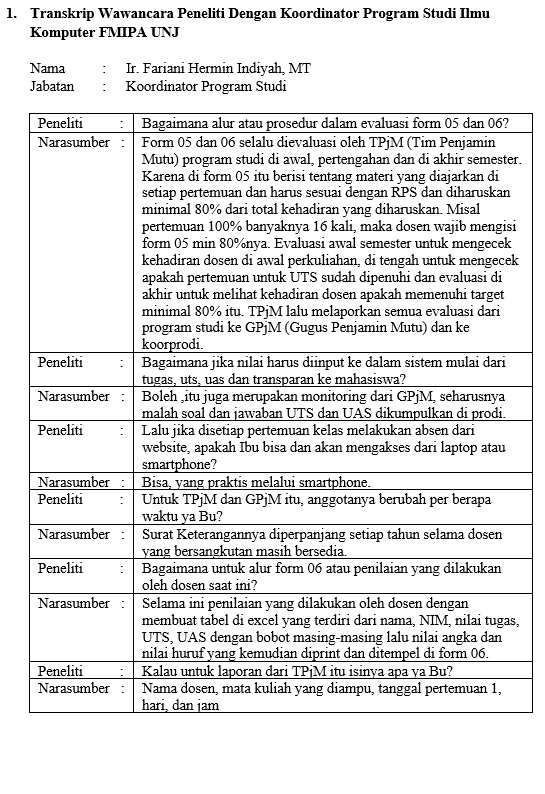
\includegraphics[width=0.9\textwidth]{gambar/lampiran/UR-1}	
\end{figure}
\begin{figure}[H]
	\centering
	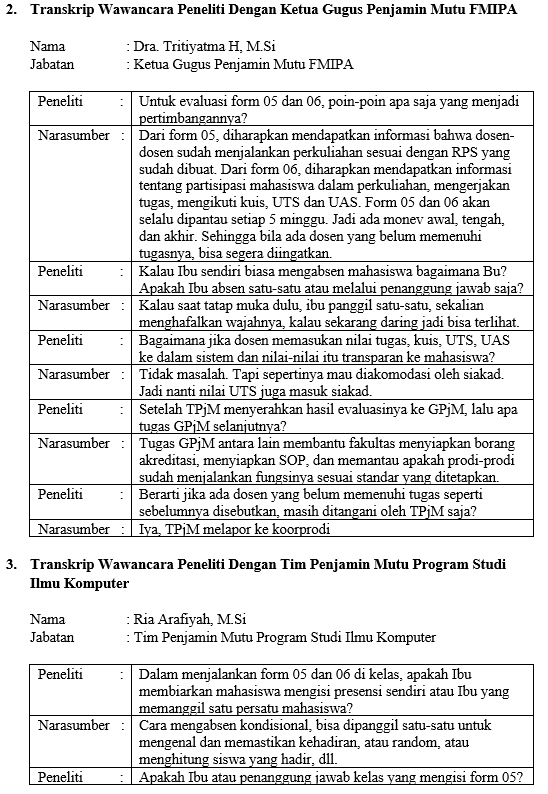
\includegraphics[width=0.9\textwidth]{gambar/lampiran/UR-2}	
\end{figure}
\begin{figure}[H]
	\centering
	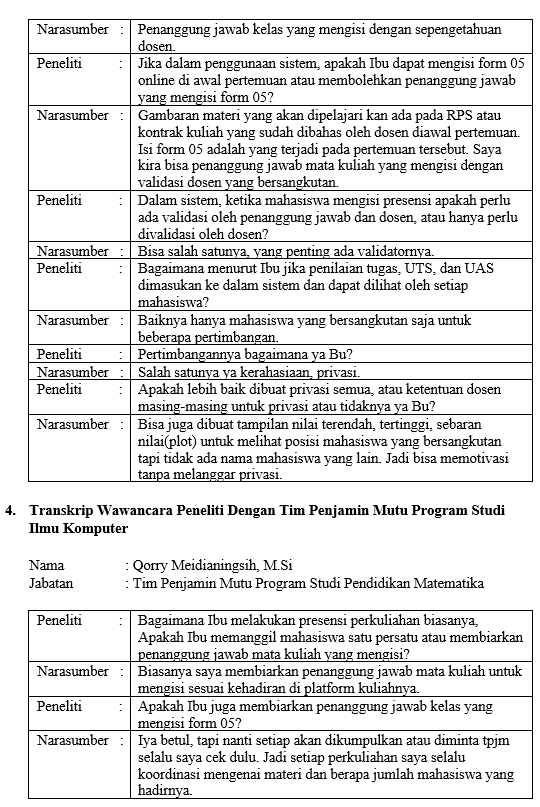
\includegraphics[width=0.9\textwidth]{gambar/lampiran/UR-3}	
\end{figure}
\begin{figure}[H]
	\centering
	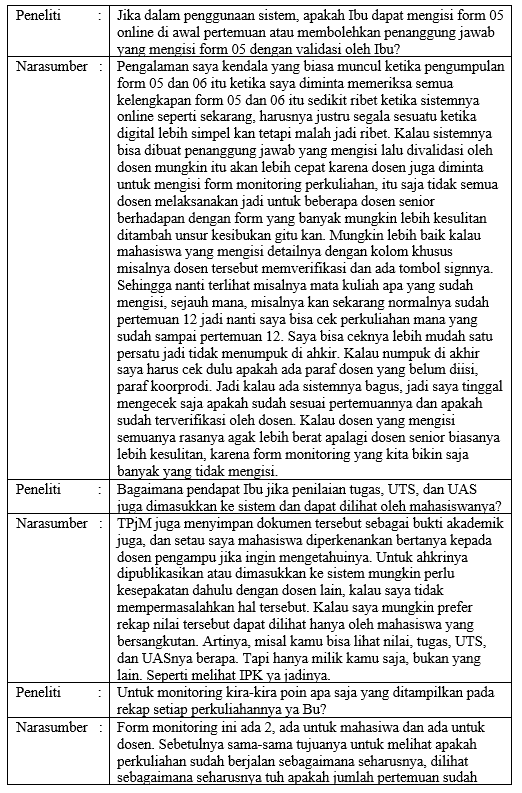
\includegraphics[width=0.9\textwidth]{gambar/lampiran/UR-4}	
\end{figure}

\begin{figure}[H]
	\centering
	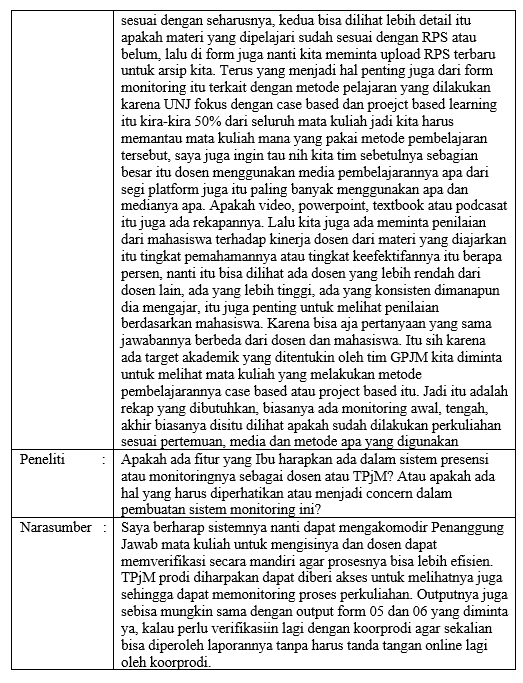
\includegraphics[width=0.9\textwidth]{gambar/lampiran/UR-5}	
\end{figure}

\chapter{Wawancara dengan Kepala UPT TIK}

\begin{figure}[H]
	\centering
	\includegraphics[width=0.9\textwidth]{gambar/lampiran/Wawancara Upt TIK}	
\end{figure}

\chapter{Sampel Kode KelasController}

\begin{lstlisting}[breaklines]
<?php

namespace App\Http\Controllers;

use App\ApiUtils\SiakadUtils;
use App\Http\Resources\KelasResourceCollection;
use App\Http\Resources\KelasDetailsResource;
use App\Http\Resources\KelasDosenResourceCollection;
use App\Http\Resources\KelasTpjmResourceCollection;
use App\Http\Resources\RekapPresensiResourceCollection;
use Illuminate\Http\Request;
use App\KelasMahasiswa;
use App\KelasDosen;
use App\RPSKelas;
use App\User;
use Validator;

class KelasController extends Controller
{
    public function __construct()
    {
        $this->middleware('auth');
    }

    public function getAllKelas($semester)
    {
        if(auth()->user()->isDosen()) {
            $resp = SiakadUtils::getKelasDosen(auth()->user()->username,$semester,auth()->user()->token_siakad);

            if($resp->status != true) return response()->json(['message' => 'Data not found!']);
            $data = collect($resp->isi);
            $diff =array_diff($data->pluck('kelas')->toArray(),auth()->user()->kelas->pluck('kelas_id')->toArray());
            if($diff) {
                foreach($diff as $item) {
                    KelasDosen::create([
                        'kelas_id' => $data->where('kelas',$item)->first()->kelas,
                        'user_id' => auth()->user()->id,
                        'semester' => $semester
                    ]);
                }
            }
            // dd($resp->isi);
            return new KelasDosenResourceCollection($resp->isi);
        } else {
            $resp = SiakadUtils::getKelasMahasiswaBySemester(auth()->user()->username,$semester,auth()->user()->token_siakad);
            if($resp->status != true) return response()->json(['message' => 'Data not found!']);
            $data = collect($resp->isi);
            $diff =array_diff($data->pluck('kelas')->toArray(),auth()->user()->kelas->pluck('kelas_id')->toArray());
            if($diff) {
                foreach($diff as $item) {
                    KelasMahasiswa::create([
                        'kelas_id' => $data->where('kelas',$item)->first()->kelas,
                        'user_id' => auth()->user()->id,
                        'semester' => $semester
                    ]);
                }
            }
            return new KelasResourceCollection($resp->isi);
        }
    }

    public function getKelas($semester,$id) {
        //kelas per seksi, cari kode prodi
        $kelas = SiakadUtils::getKelasInfo($id,$semester,auth()->user()->token_siakad);

        if($kelas->status == false) return response()->json(['message' => 'Kelas tidak ditemukan']);
        $kode_prodi = $kelas->identitas->kode_prodi;
        $kelas = collect(SiakadUtils::getKelasInProdi($kode_prodi,auth()->user()->prodi->fakultas->kode,$semester));

        return new KelasDetailsResource(collect($kelas['isi'])->where('kelas',$id)->first());
    }

    public function getKelasHariIni($semester) {
        if(auth()->user()->isDosen()) {
            $resp = SiakadUtils::getKelasDosen(auth()->user()->username,$semester,auth()->user()->token_siakad);

            if($resp->status != true) return response()->json(['message' => 'Data not found!']);
            $data = collect($resp->isi);
            $data = $data->where('hari',\Carbon\Carbon::now()->isoFormat('d'));
            $diff =array_diff($data->pluck('kelas')->toArray(),auth()->user()->kelas->pluck('kelas_id')->toArray());
            if($diff) {
                foreach($diff as $item) {
                    KelasDosen::create([
                        'kelas_id' => $data->where('kelas',$item)->first()->kelas,
                        'user_id' => auth()->user()->id,
                        'semester' => $semester
                    ]);
                }
            }
            // dd($resp->isi);
            return new KelasDosenResourceCollection($data);
        } else {
            $resp = SiakadUtils::getKelasMahasiswaBySemester(auth()->user()->username,$semester,auth()->user()->token_siakad);
            if($resp->status != true) return response()->json(['message' => 'Data not found!']);
            $data = collect($resp->isi);
            $data = $data->where('hari',\Carbon\Carbon::now()->isoFormat('d'));
            $diff =array_diff($data->pluck('kelas')->toArray(),auth()->user()->kelas->pluck('kelas_id')->toArray());
            if($diff) {
                foreach($diff as $item) {
                    KelasMahasiswa::create([
                        'kelas_id' => $data->where('kelas',$item)->first()->kelas,
                        'user_id' => auth()->user()->id,
                        'semester' => $semester
                    ]);
                }
            }
            return new KelasResourceCollection($data);
        }
    }

    public function uploadRPS($id, Request $request)
    {
        $validator = Validator::make($request->all(),
        [
        'file' => 'required|mimes:pdf|max:2048',
       ]);

        if ($validator->fails()) {
            return response()->json(['error'=>$validator->errors()], 415);
        }

        if ($files = $request->file('file')) {

            //store file into document folder
            $originalName = $request->file->getClientOriginalName();
            $file = $request->file->storeAs('public\\rps',$originalName);

            //store your file into database
            $existing = RPSKelas::where('kelas_id',$id)->first();
            if($existing) {
                $existing->filename = $originalName;
                $existing->save();
            } else {
                RPSKelas::create([
                    'filename' => $originalName,
                    'kelas_id' => $id
                ]);
            }

            return response()->json([
                "success" => true,
                "message" => "File successfully uploaded",
                "file" => $file
            ],200);
        }
    }

    public function downloadRPS($id, Request $request)
    {
        $rps = RPSKelas::where('kelas_id',$id)->first();
        if($rps == null) {
            return response()->json([
                'message' => 'File not found'
            ],404);
        }

        $file= public_path(). config('storage.path') . $rps->filename;

        $headers = array(
            'Content-Type: application/pdf',
        );
        return response()->download($file, 'filename.pdf', $headers);
    }

    public function getAllKelasInProdi($semester)
    {
        $prodi = auth()->user()->prodi;
        $fakultas = $prodi->fakultas;
        $resp = SiakadUtils::getKelasInProdi($prodi->kode,$fakultas->kode,$semester);
        if($resp->status != true) return response()->json(['message' => 'Data not found!']);
        $data = collect($resp->isi);

        return new KelasTpjmResourceCollection($data);
    }

    public function assignPJ($semester,$id,Request $request)
    {
        if(!auth()->user()->isDosen() || auth()->user()->kelas->where('kelas_id',$id)->where('semester',$semester)->isEmpty()) return response()->json(['message' => 'Unauthorized!'],401);

        $mhs_id = User::where('username',$request->mahasiswa)->first()->id;
        $pivot = KelasMahasiswa::where('kelas_id', $id)->where('user_id',$mhs_id)->where('semester',$semester)->first();
        $pivot->penanggung_jawab = 1;
        $pivot->save();

        return response()->json(['message' => 'Success!'],200);
    }

    public function getMahasiswaList($semester,$id)
    {
        $mahasiswa_id = KelasMahasiswa::where('kelas_id',$id)->where('semester',$semester)->get()->map->only('user_id','penanggung_jawab');
        $listLengkap = $mahasiswa_id->map(function ($item,$key) {
            $user = User::find($item['user_id']);
            return [
                    'username' => $user->username,
                    'nama'=> $user->nama,
                    'penanggung_jawab'=> $item['penanggung_jawab']];
        });
        return $listLengkap;
    }

    public function rekapPresensi($semester)
    {
        $resp = SiakadUtils::getKelasMahasiswaBySemester(auth()->user()->username,$semester,auth()->user()->token_siakad);
        if($resp->status != true) return response()->json(['message' => 'Data not found!']);
        $data = collect($resp->isi);
        return new RekapPresensiResourceCollection($data);
    }
}
\end{lstlisting}

\chapter{Sampel Kode View Form05}

\begin{lstlisting}[breaklines]
<template>
  <!-- Content Wrapper. Contains page content -->

  <div class="tab-pane fade show active" id="custom-content-below-home" role="tabpanel"
    aria-labelledby="custom-content-below-home-tab">
    <br>
    <!-- Main content -->
    <section class="content">
      <div class="container-fluid">
        <div v-if="kelas_info" class="row">
          <div class="col-2-md">
            <button v-if="(kelas_info.is_penanggung_jawab || isDosen) && !isMonitoring  && isSemesterAktif" type="button" class="btn btn-primary"
              @click.prevent="tambahPertemuan">
              <!-- <button type="button" class="btn btn-primary" data-toggle="modal" data-target="#modal-lg"> -->
              Pertemuan Baru
            </button>
          </div>
          <div class="ml-auto">
            <button @click="callForm05()" type="button" class="btn btn-secondary">
              <span v-if="!loading" class="fa fa-sync"></span>
              <span v-if="loading" class="spinner-border spinner-border-sm" role="status" aria-hidden="true"></span>
              <span v-if="loading" class="sr-only">Loading...</span>
            </button>
          </div>
        </div>
        <br />
        <div class="row">
          <div class="col-md-12">
            <div class="card">
              <!-- <div class="card-header">
                <h3 class="card-title">Form 05</h3>
              </div> -->
              <div class="card-body table-responsive">
                <table class="table table-bordered table-hover">
                  <thead>
                    <tr>
                      <th style="width: 10px">Pertemuan</th>
                      <th>Waktu</th>
                      <th>Materi</th>
                      <th>Jumlah Mahasiswa Hadir</th>
                      <th>Validasi Dosen</th>
                      <th>Validasi Mahasiswa</th>
                      <th v-if="!isMonitoring  && isSemesterAktif">Action</th>
                    </tr>
                  </thead>
                  <tbody>
                    <tr v-for="(form, index) in form05" :key="form.id">
                      <td>{{ form.pertemuan }}</td>
                      <td>{{ form.created_at }}</td>
                      <td>{{ form.materi }}</td>
                      <td>{{ form.jumlah_mahasiswa }}</td>
                      <td>
                        <i v-show="form.valid_dosen == true" class="fas fa-check"></i>
                        <button @click="validasiPertemuan(form.id, index)" v-show="form.valid_dosen == false && isDosen && !isMonitoring  && isSemesterAktif"
                          type="button" class="btn btn-primary">
                          Validasi
                        </button>
                        <span v-show="form.valid_dosen == false && (!isDosen || isMonitoring || !isSemesterAktif)">Waiting...</span>
                      </td>
                      <td>
                        <i v-show="form.valid_mahasiswa == true" v-tooltip="form.penanggung_jawab" class="fas fa-check"></i>
                        <button @click="validasiPertemuan(form.id, index)" v-show="form.valid_mahasiswa == false && !isDosen  && isSemesterAktif && (kelas_info.is_penanggung_jawab || form.penanggung_jawab == username)"
                          type="button" class="btn btn-primary">
                          Validasi
                        </button>
                        <span v-show="form.valid_mahasiswa == false && (isDosen || !(kelas_info.is_penanggung_jawab || form.penanggung_jawab == username) )">Waiting...</span>
                      </td>
                      <td v-if="isDosen && !isMonitoring && isSemesterAktif">
                        <button type="button" @click="ubahMateri(form.id,index)" class="btn btn-success">Ubah
                          materi</button>
                        <button type="button" @click="modalValidasi(form.id)" class="btn btn-primary">Validasi
                          Presensi</button>
                        <button type="button" class="btn btn-secondary" @click="modalPJSementara(form.id,index)">Penanggung Jawab Sementara</button>
                        <button type="button" class="btn btn-warning" @click="modalPerizinan(form.id)">Perizinan</button>
                        <button type="button" class="btn btn-danger" @click="hapusForm(form.id,index)"><span class="fa fa-trash"></span></button>
                      </td>
                      <td v-else-if="!isMonitoring && isSemesterAktif">
                        <div v-if="checkWaktu(form.created_at)">
                          <button v-if="form.hadir == false || (form.hadir && form.hadir_valid)" :disabled="form.hadir" @click="hadirPertemuan(form.id,index)" type="button"
                            class="btn btn-primary">Hadir</button>
                          <button v-else-if="form.izin == true" @click="hadirPertemuan(form.id,index)" type="button" disabled
                            class="btn btn-warning">Izin</button>
                          <button v-else-if="form.hadir == true && form.hadir_valid == false" @click="hadirPertemuan(form.id,index)" type="button" disabled
                            class="btn btn-secondary">Menunggu validasi kehadiran</button>
                        </div>
                        <div v-else>
                        <button v-if="form.hadir && form.hadir_valid" disabled type="button"
                          class="btn btn-primary">Hadir</button>
                          <button v-if="form.izin == true" @click="hadirPertemuan(form.id,index)" type="button" disabled
                            class="btn btn-warning">Izin</button>
                        <button v-else disabled type="button"
                          class="btn btn-danger">Tidak Hadir</button>
                        </div>
                        <button v-if="kelas_info.is_penanggung_jawab || form.penanggung_jawab == username" @click="modalValidasi(form.id)" type="button"
                          class="btn btn-info">Validasi Presensi</button>
                      </td>
                    </tr>
                    <tr v-show="form05.length == 0">
                      <td colspan="8" style="text-align:center">
                        <div v-if="loading" class="spinner-border text-primary" role="status">
                          <span class="sr-only">Loading...</span>
                        </div>
                        <div v-if="!loading">No Data</div>
                      </td>
                    </tr>
                  </tbody>
                </table>
              </div>
            </div>
          </div>
        </div>
      </div>
    </section>
    <!-- /.content -->
    <div v-show="show_modal">
      <transition name="modal">
        <div class="modal-mask" >
          <div class="modal-wrapper" @click.self="show_modal=false">
            <div class="modal-dialog" ref="modal_validasi" tabindex="0" @keyup.esc="show_modal=false">
              <div v-if="show_modal" class="modal-content">
                <div class="modal-header">
                  <h4 class="modal-title">Validasi Presensi</h4>
                  <button type="button" class="close" @click="show_modal=false">
                    <span aria-hidden="true">&times;</span>
                  </button>
                </div>
                <div class="modal-body">
                  <div class="table-responsive" style="max-height: 300px;">
                    <table class="table table-head-fixed">
                      <thead>
                        <tr>
                          <th style="text-align:center">Nama Mahasiswa</th>
                          <th style="text-align:center">Waktu</th>
                          <th style="text-align:center">Validasi</th>
                        </tr>
                      </thead>
                      <tbody v-if="!modalLoading">
                        <tr v-if="listPresensi.length != 0" @click="checkboxAllToggle()" style="cursor:pointer;">
                          <td colspan="2" style="text-align:center;vertical-align:middle"> Validasi Semua</td>
                          <td style="text-align:center;vertical-align:middle">
                            <input style="cursor:pointer" type="checkbox"  id="checkbox_all" v-model="checkboxAll">
                          </td>
                        </tr>
                        <tr v-else>
                          <td colspan="3" style="text-align:center">
                            <div >No Data</div>
                          </td>
                        </tr>
                        <tr v-for="list in listPresensi" :key="list.id" style="height:60px;cursor:pointer;" @click="clickValidasi(list.id)" >
                          <td style="text-align:center;vertical-align:middle">{{list.nama}}</td>
                          <td style="text-align:center;vertical-align:middle">{{list.waktu}}</td>
                          <td style="text-align:center;vertical-align:middle">
                            <input style="cursor:pointer" type="checkbox" :value="list.id" :id="'checkbox_'+list.id" v-model="listValidasi">
                          </td>
                        </tr>
                      </tbody>
                      <tbody v-else>
                        <tr>
                          <td colspan="3" style="text-align:center">
                            <div class="spinner-border text-primary" role="status">
                              <span class="sr-only">Loading...</span>
                            </div>
                          </td>
                        </tr>
                      </tbody>
                    </table>
                  </div>
                </div>
                <div class="modal-footer" v-show="listPresensi.length != 0">
                 <button type="button" class="btn btn-primary" @click="validasiPresensi()">Validasi</button>
                </div>
              </div>
            </div>
          </div>
        </div>
      </transition>
    </div>
    <!-- Modal PJ sementara -->
    <div v-show="show_modal_pj">
      <transition name="modal">
        <div class="modal-mask" >
          <div class="modal-wrapper" @click.self="show_modal_pj=false">
            <div class="modal-dialog" ref="modal_pj" tabindex="0" @keyup.esc="show_modal_pj=false">
              <div v-if="show_modal_pj" class="modal-content">
                <div class="modal-header">
                  <h4 class="modal-title">Pilih Penangung Jawab</h4>
                  <button type="button" class="close" @click="show_modal_pj=false">
                    <span aria-hidden="true">&times;</span>
                  </button>
                </div>
                <div class="modal-body">
                  <v-select label="nama" v-model="penanggungJawabSementara" :options="listMahasiswa" :dropdown-should-open="dropdownShouldOpen"></v-select>
                </div>
                <div class="modal-footer">
                 <button type="button" class="btn btn-primary" @click="assignPJ()">Pilih</button>
                </div>
              </div>
            </div>
          </div>
        </div>
      </transition>
    </div>
    <!-- Modal Perizinan -->
    <div v-show="show_modal_perizinan">
      <transition name="modal">
        <div class="modal-mask" >
          <div class="modal-wrapper" @click.self="show_modal_perizinan=false">
            <div class="modal-dialog" ref="modal_perizinan" tabindex="0" @keyup.esc="show_modal_perizinan=false">
              <div v-if="show_modal_perizinan" class="modal-content">
                <div class="modal-header">
                  <h4 class="modal-title">Masukan nama mahasiswa dengan izin</h4>
                  <button type="button" class="close" @click="show_modal_perizinan=false">
                    <span aria-hidden="true">&times;</span>
                  </button>
                </div>
                <div class="modal-body">
                  <v-select multiple label="nama" v-model="perizinanMahasiswa" :options="listMahasiswa" :dropdown-should-open="dropdownShouldOpen"></v-select>
                </div>
                <div class="modal-footer">
                 <button type="button" class="btn btn-primary" @click="perizinan()">Pilih</button>
                </div>
              </div>
            </div>
          </div>
        </div>
      </transition>
    </div>
    <!-- /.modal -->
    <!-- /.content-wrapper -->
  </div>
</template>
\end{lstlisting}